\graphicspath{{chapters/loadings/}}
\chapter{HCP and ADNI Loadings}\label{appendix:loadings}

This appendix builds upon the results presented in Chapter \ref{ch:als}, where we introduced a method to regularize CCA using structured priors on model weights, demonstrated with Human Connectome Project (HCP) and Alzheimer's Disease Neuroimaging Initiative (ADNI) data. In light of the insights gained from Chapter \ref{ch:loadings}, which examined the relationship between loadings and weights in CCA using simulated data, we revisit the HCP and ADNI results to further explore the interpretability of the models.


\section{Human Connectome Project (\acrshort{hcp}) Data}

This section presents the loadings for the HCP data, which were obtained using the models described in Chapter \ref{ch:als}. The loadings are visualized using chord diagrams for each model. The chord diagrams show the top 8 positive and negative brain loadings for each model. The loadings are ordered by their absolute value, with the largest loadings at the top of the diagram. The chord diagrams provide a visual representation of the relationship between the brain regions and the latent variables in each model. The loadings are color-coded to indicate the strength and direction of the relationship between the brain regions and the latent variables. Positive loadings are shown in blue, and negative loadings are shown in red. The width of the chords indicates the strength of the relationship between the brain regions and the latent variables. The chord diagrams provide a concise and intuitive way to compare the loadings across the different models and identify patterns in the relationships between the brain regions and the latent variables.

\subsection{Brain Connectivity Weights and Loadings}

Figure \ref{fig:chord_loadings} shows chord diagrams of the top 8 positive and negative brain \gls{loadings} for each model. 

\begin{figure}
    \centering
    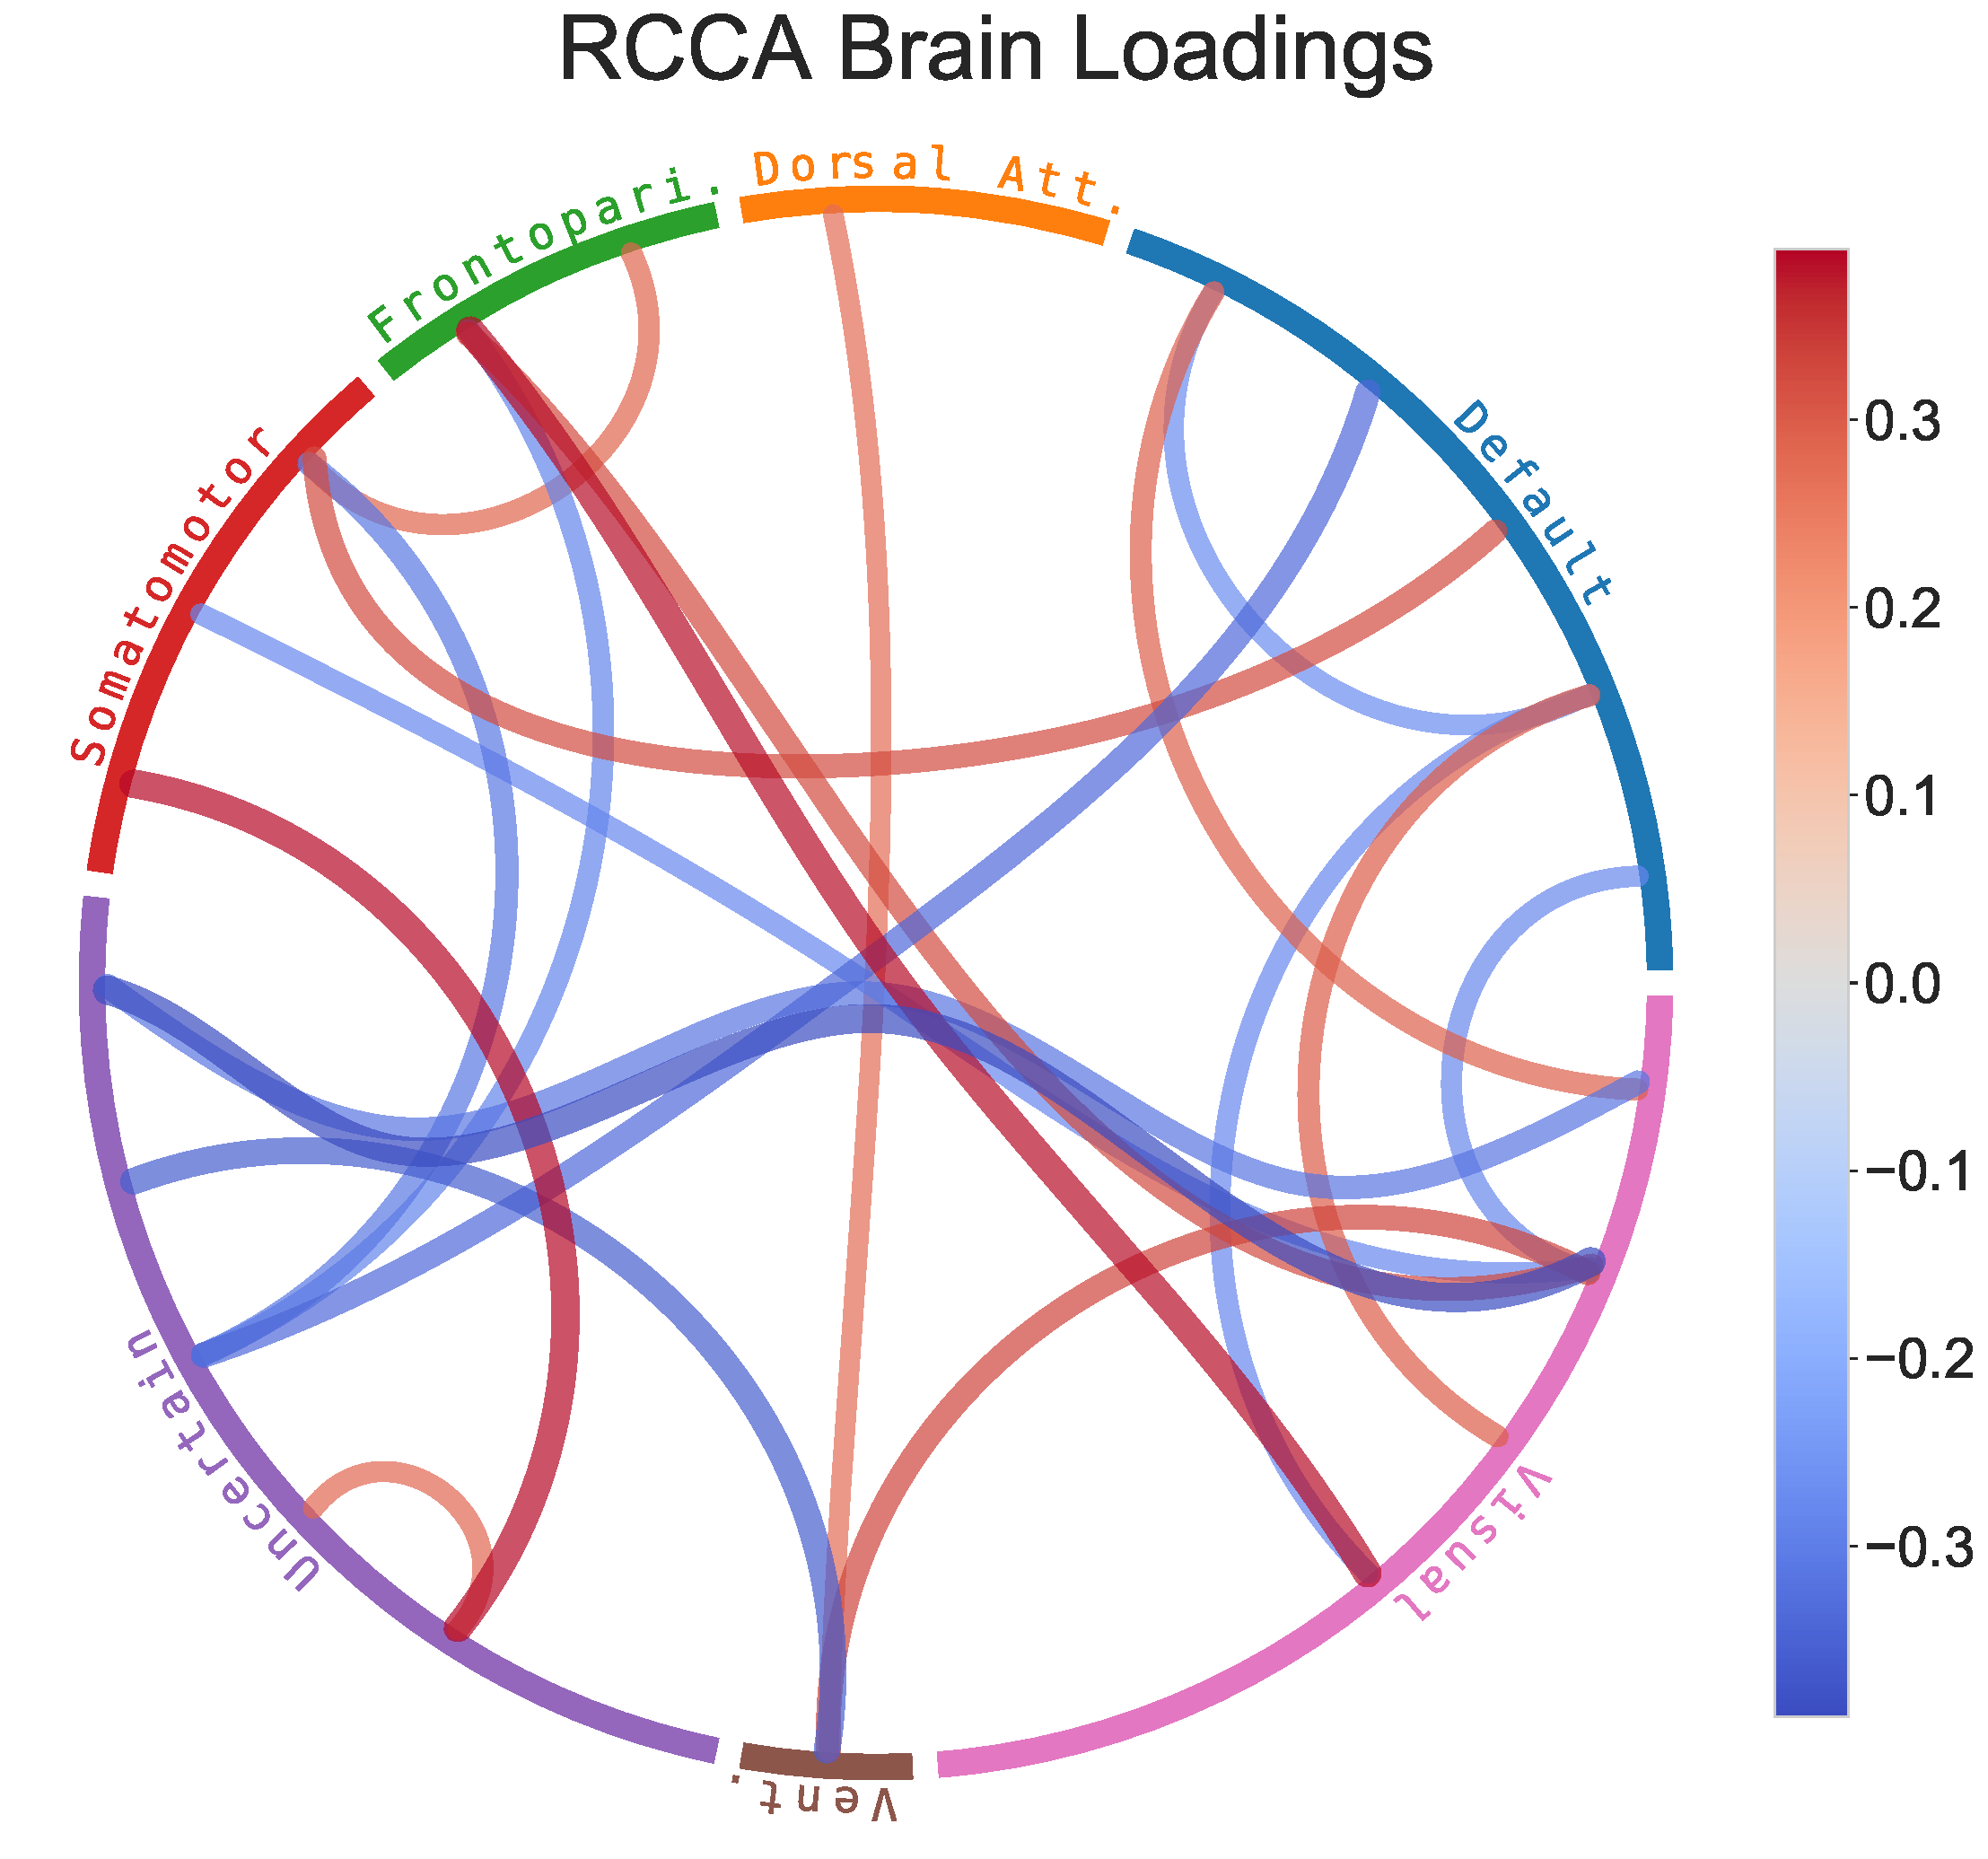
\includegraphics[width=0.49\linewidth]{figures/hcp/RCCA brain loadings}
    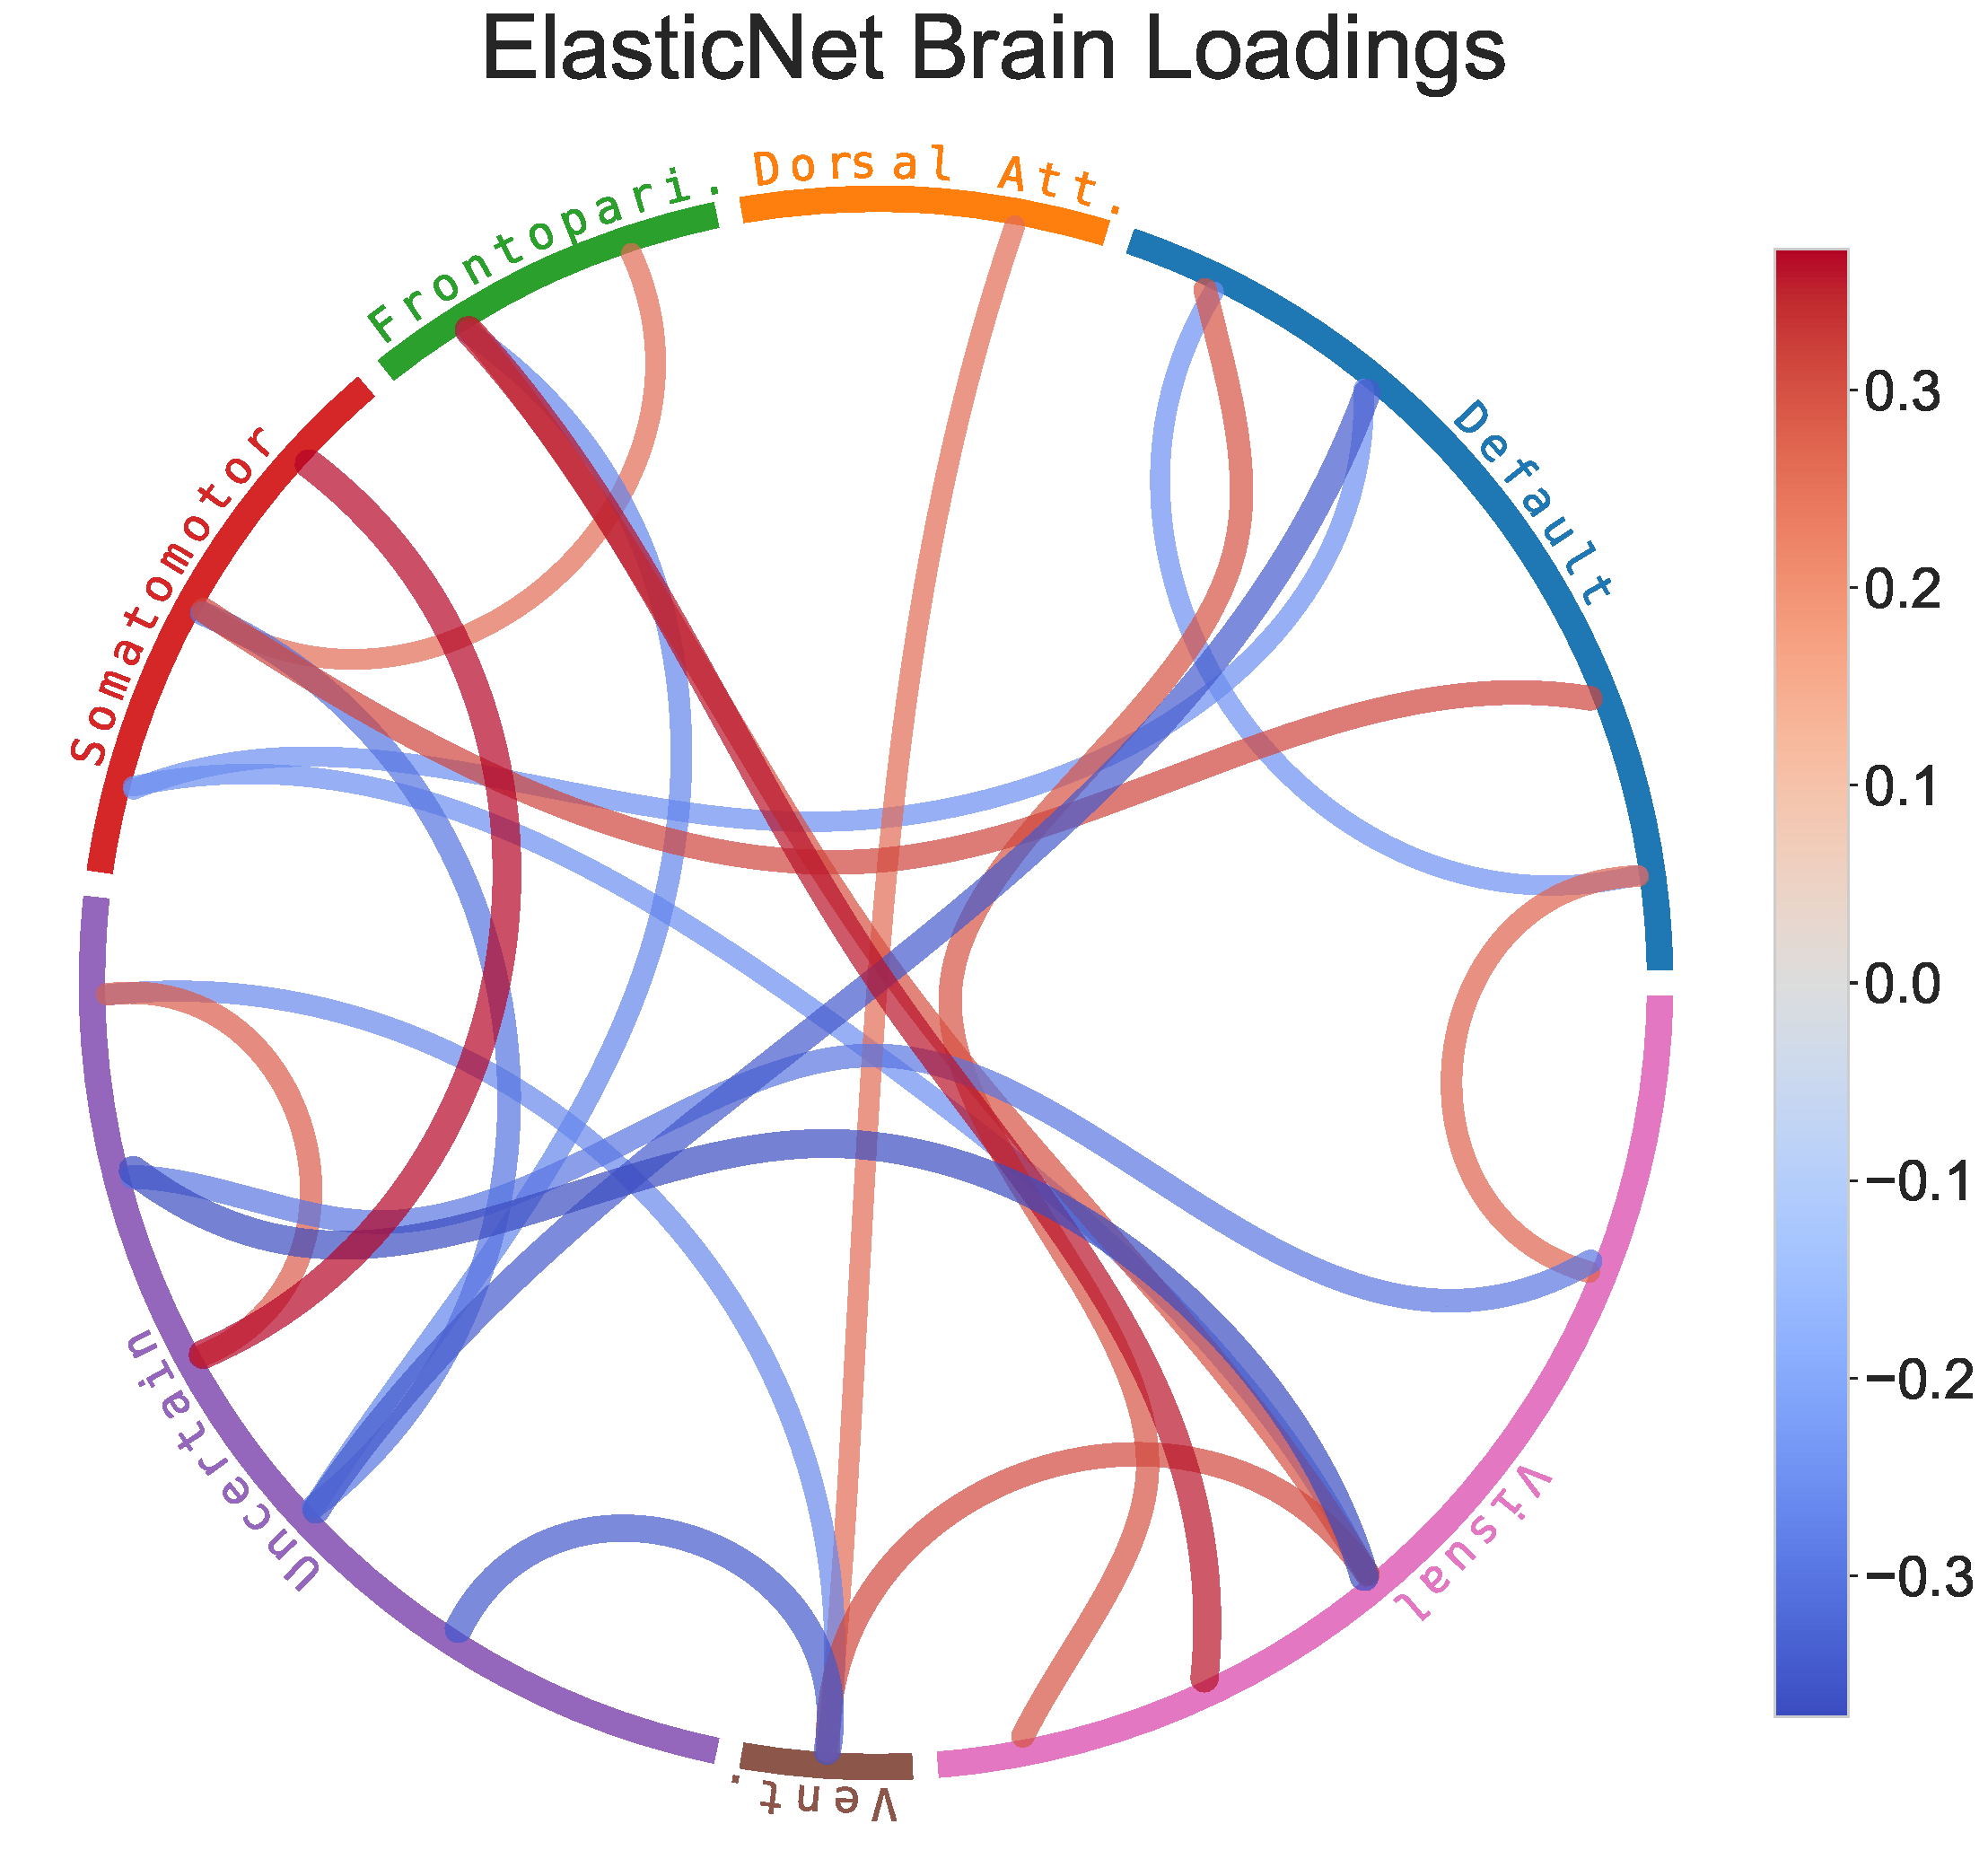
\includegraphics[width=0.49\linewidth]{figures/hcp/ElasticNet brain loadings}
    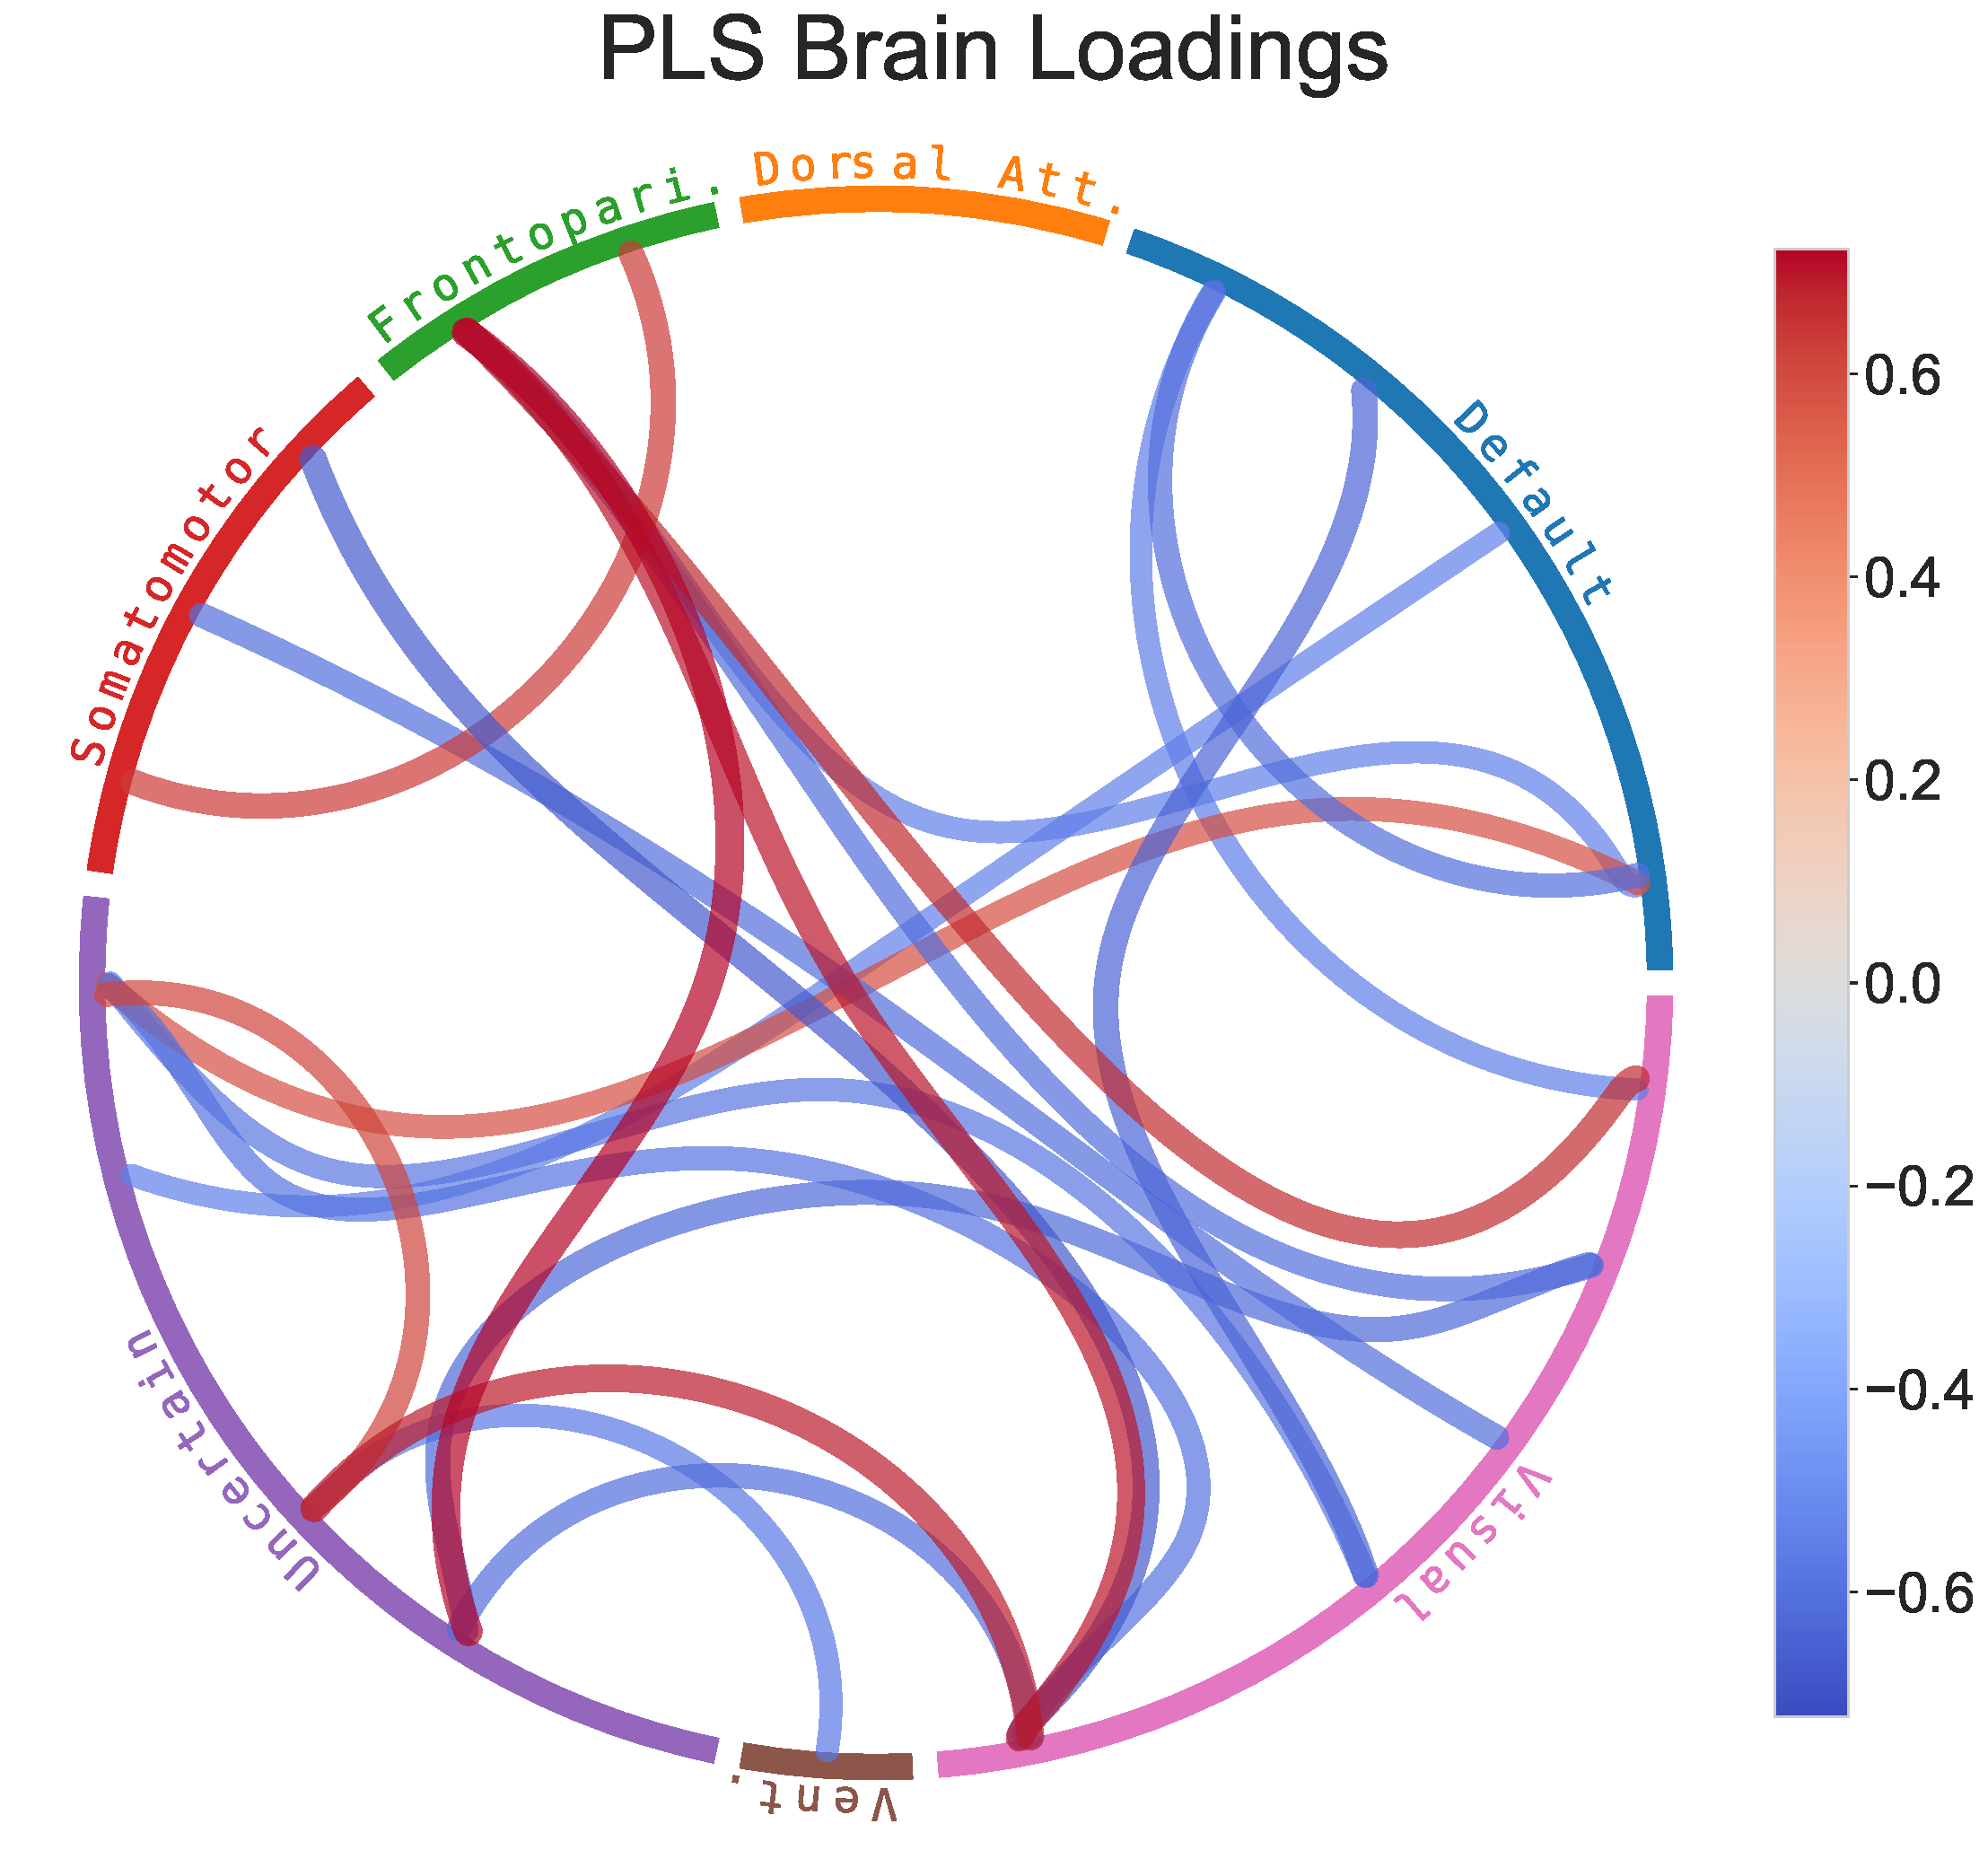
\includegraphics[width=0.49\linewidth]{figures/hcp/PLS brain loadings}
    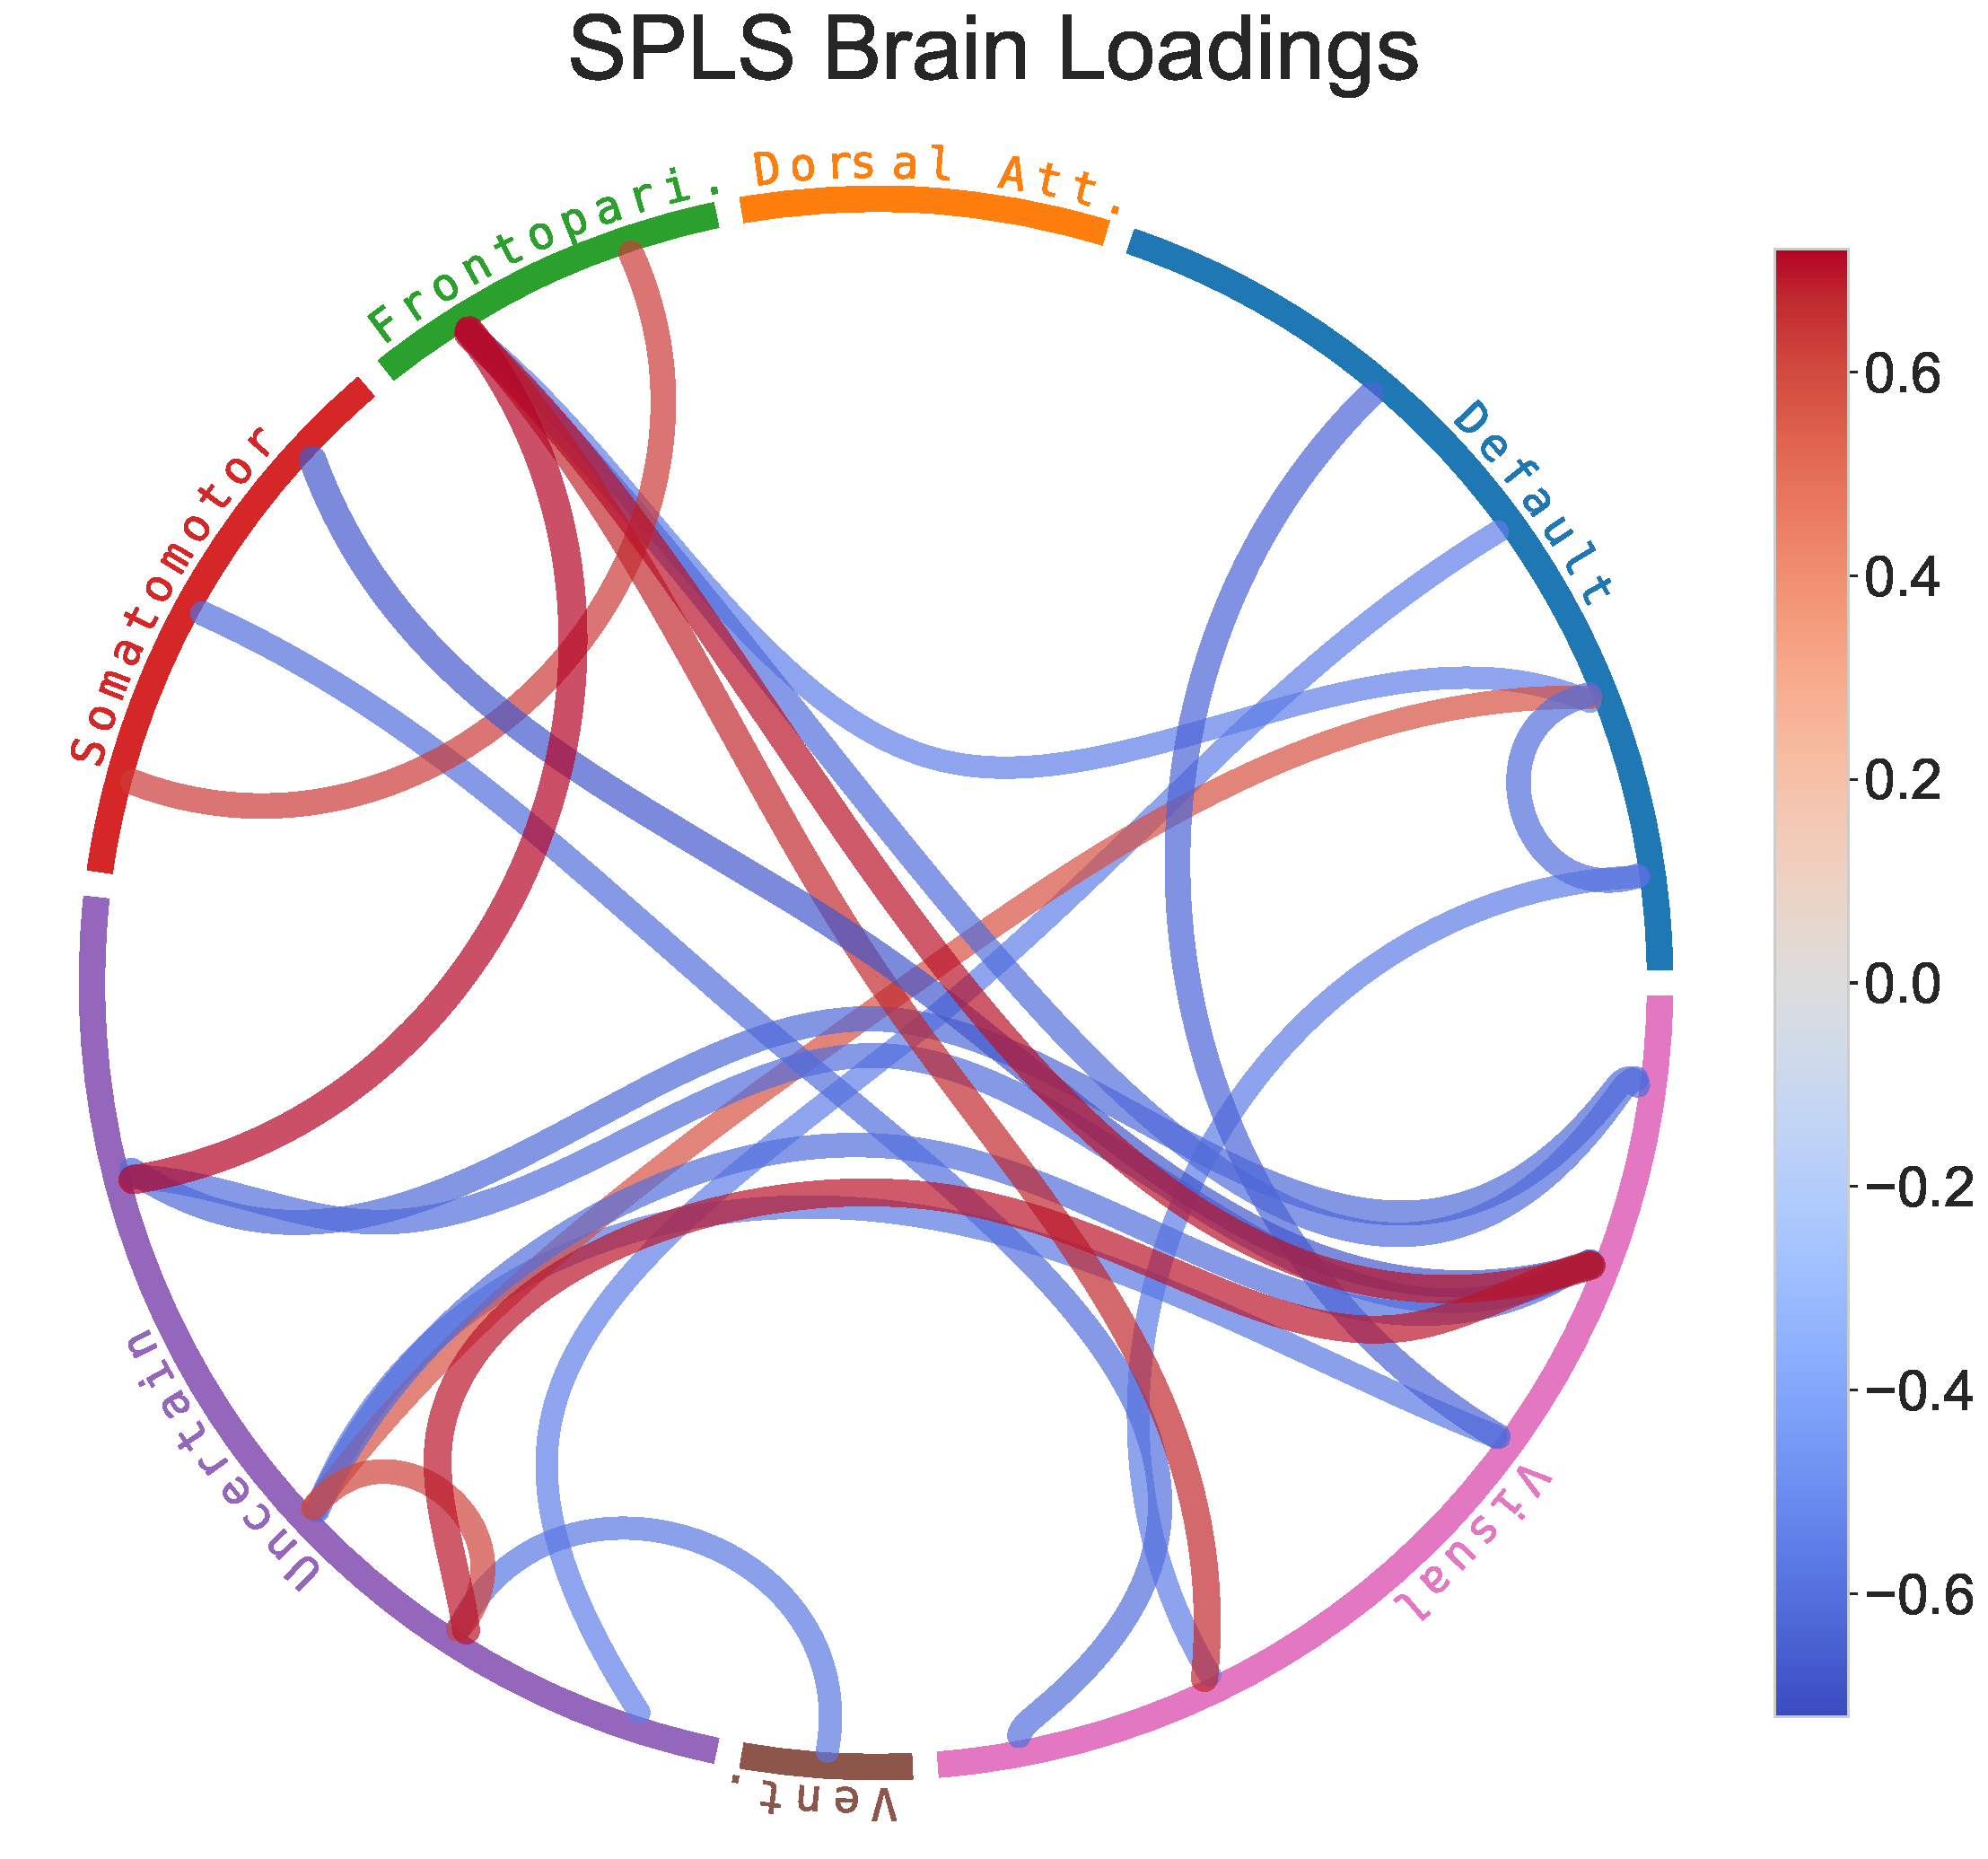
\includegraphics[width=0.49\linewidth]{figures/hcp/SPLS brain loadings}
    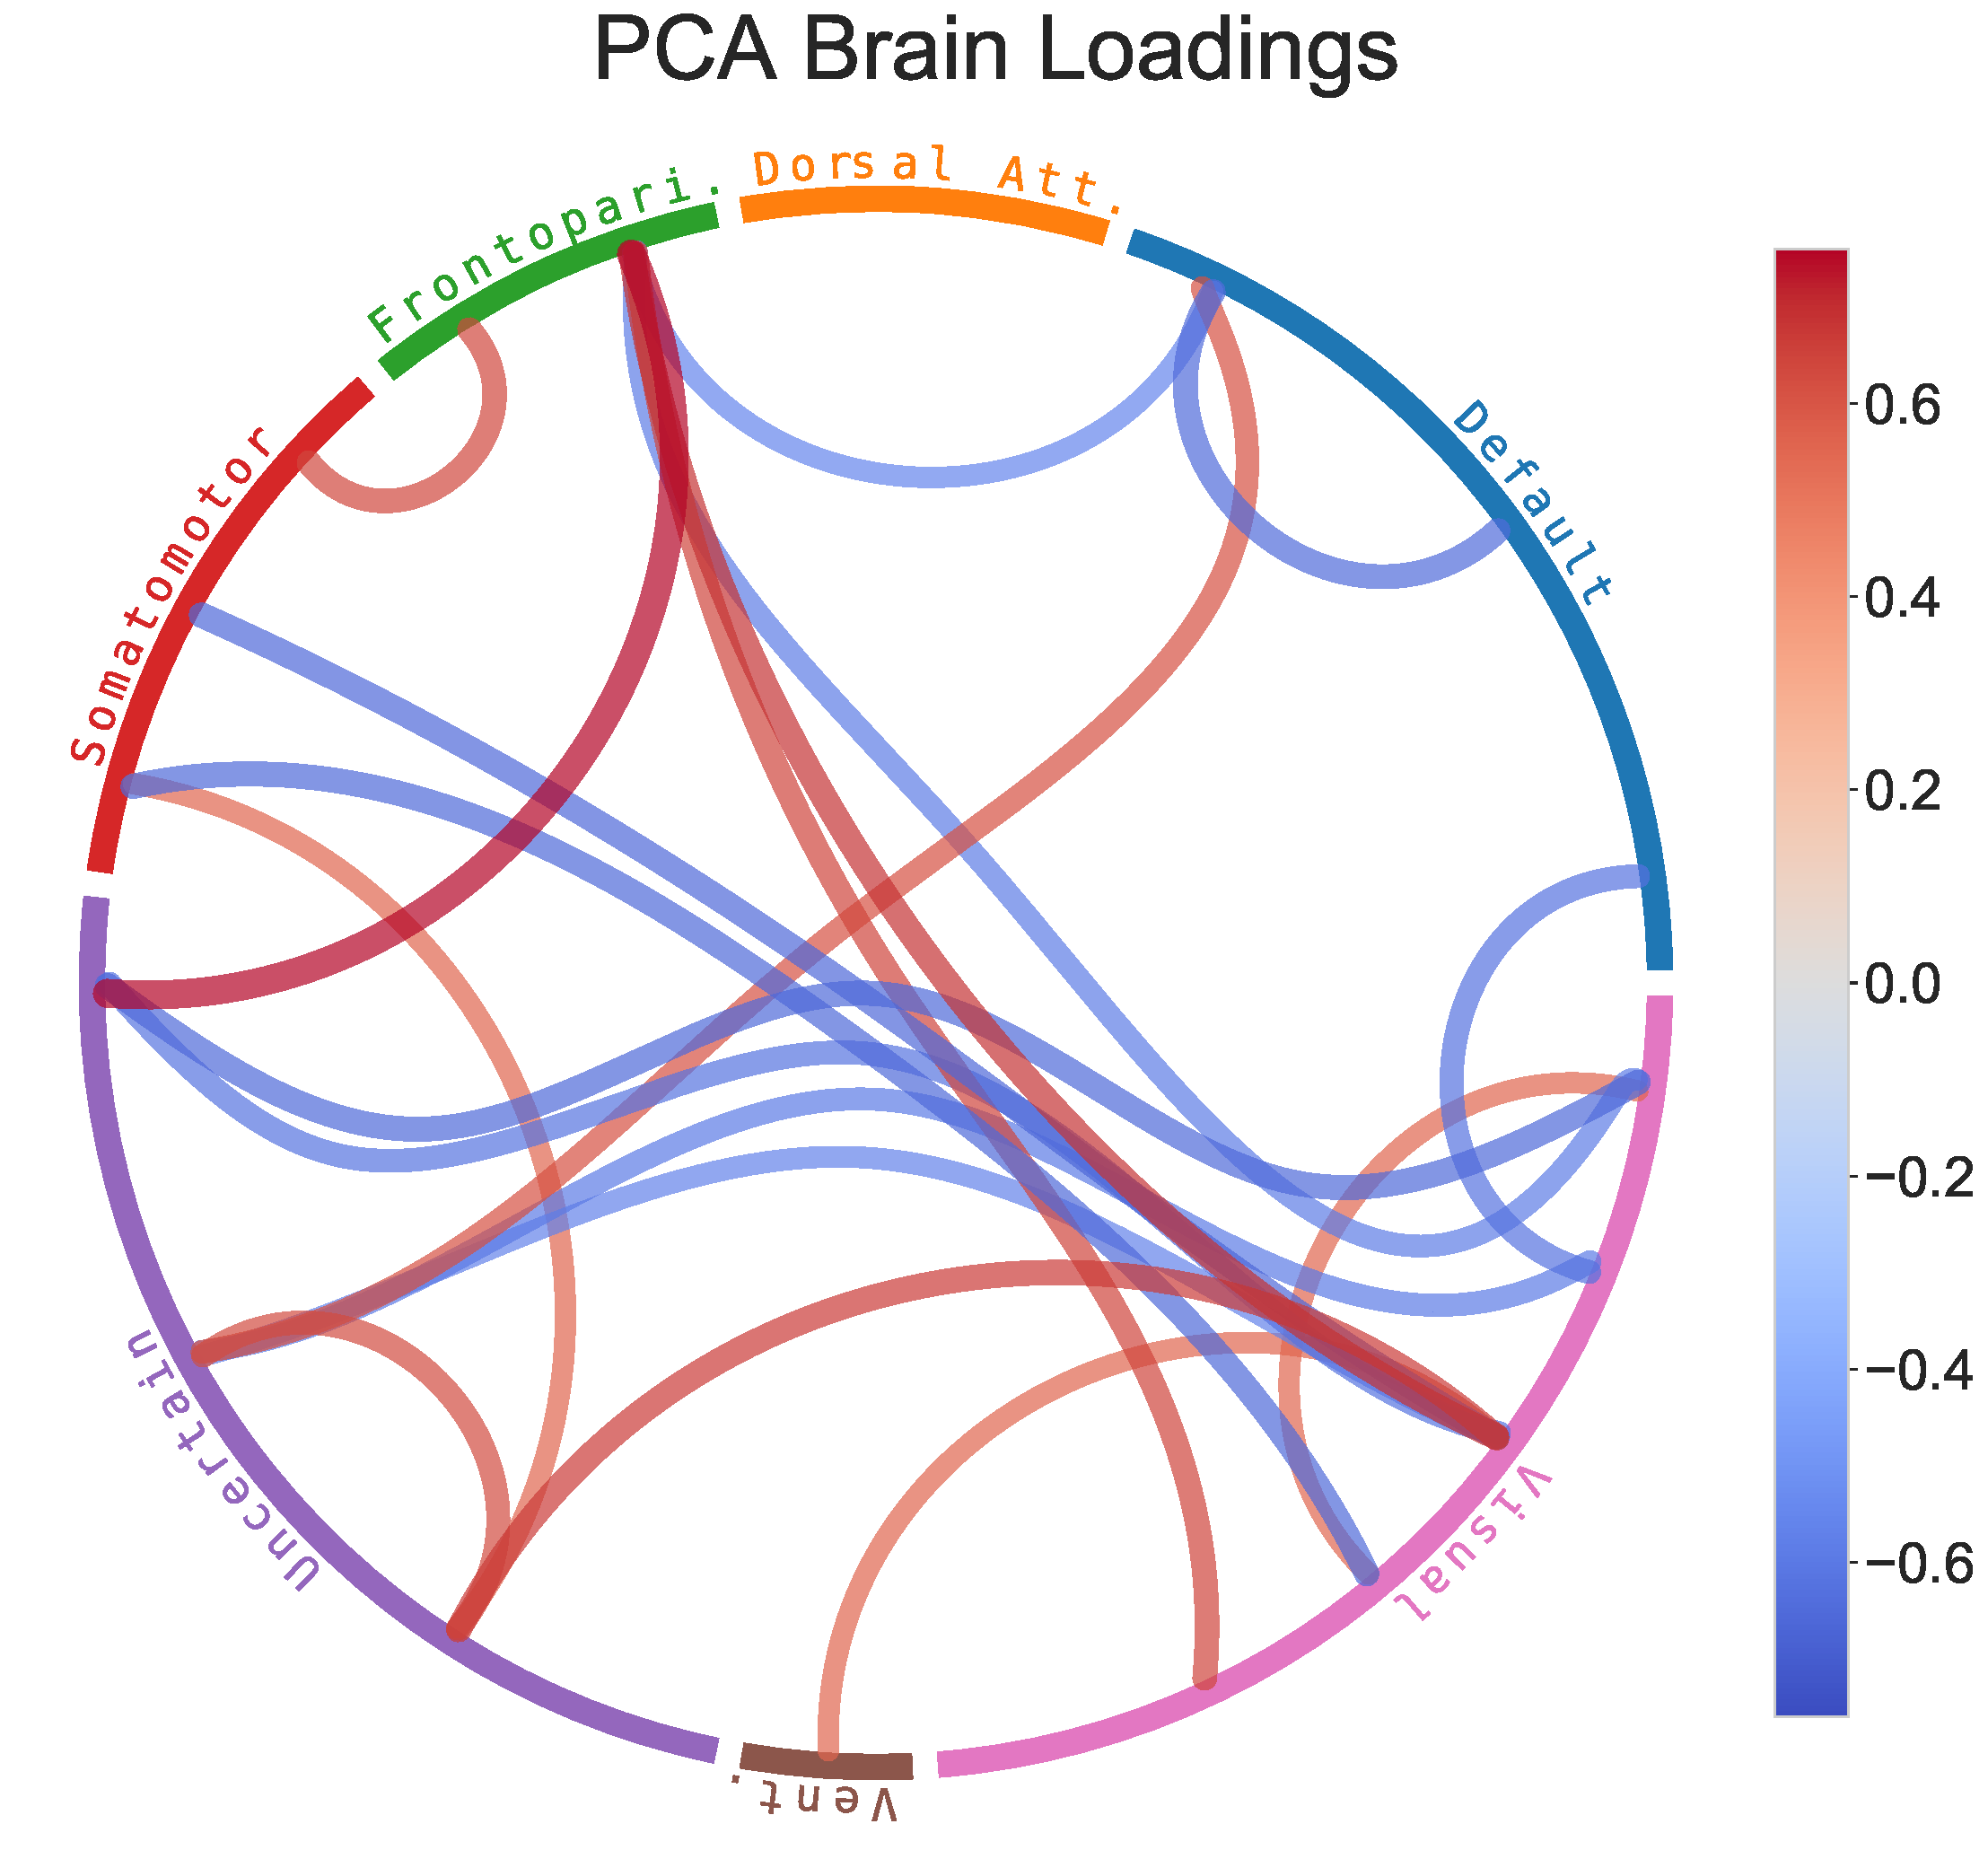
\includegraphics[width=0.49\linewidth]{figures/hcp/PCA brain loadings}
    \caption{Chord diagrams of the top 8 positive and negative brain \gls{loadings} for each model.}\label{fig:chord_loadings}
\end{figure}

\newpage


\section{Alzheimer's Disease Neuroimaging Initiative (\acrshort{adni}) Data}

This section presents the loadings for the ADNI data, which were obtained using the models described in Chapter \ref{ch:als}. The loadings are visualized using statistical maps for each model. The statistical maps show the brain structure \gls{loadings} for each model. The loadings are color-coded to indicate the strength and direction of the relationship between the brain structures and the latent variables. Positive loadings are shown in blue, and negative loadings are shown in red. The statistical maps provide a visual representation of the relationship between the brain structures and the latent variables in each model. The maps allow us to compare the loadings across the different models and identify patterns in the relationships between the brain structures and the latent variables.

\subsection{Brain Structure Weights and Loadings}

Figure \ref{fig:adni-brain} shows statistical maps of brain structure \gls{loadings} and \gls{weights} for each model.

\begin{figure}
    \centering
    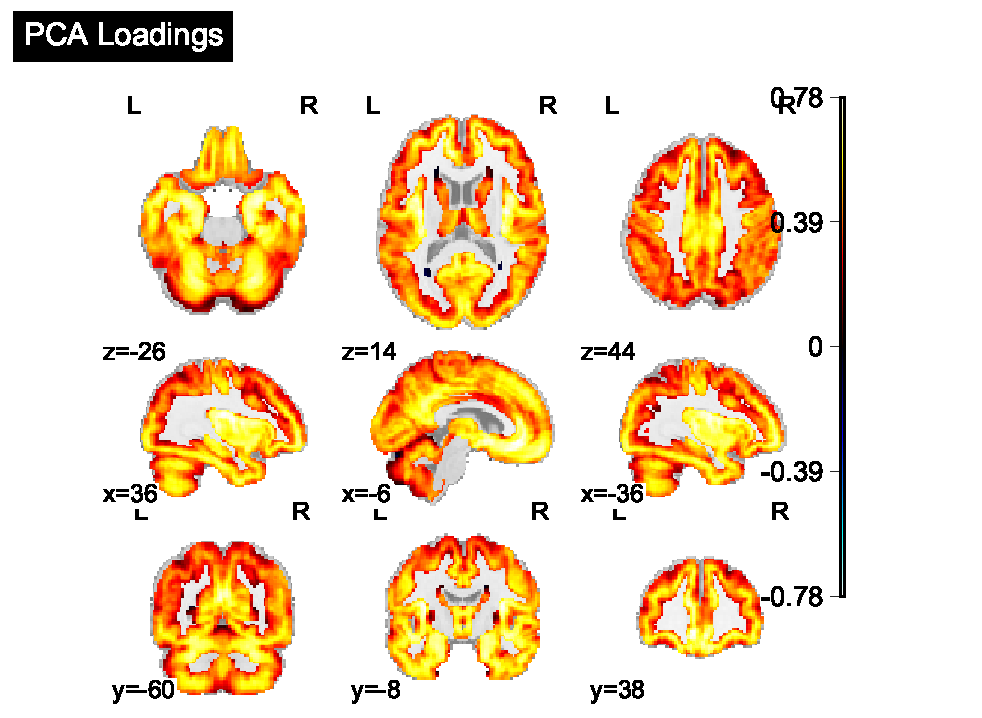
\includegraphics[width=0.45\linewidth]{figures/adni/PCA brain loadings mosaic}
    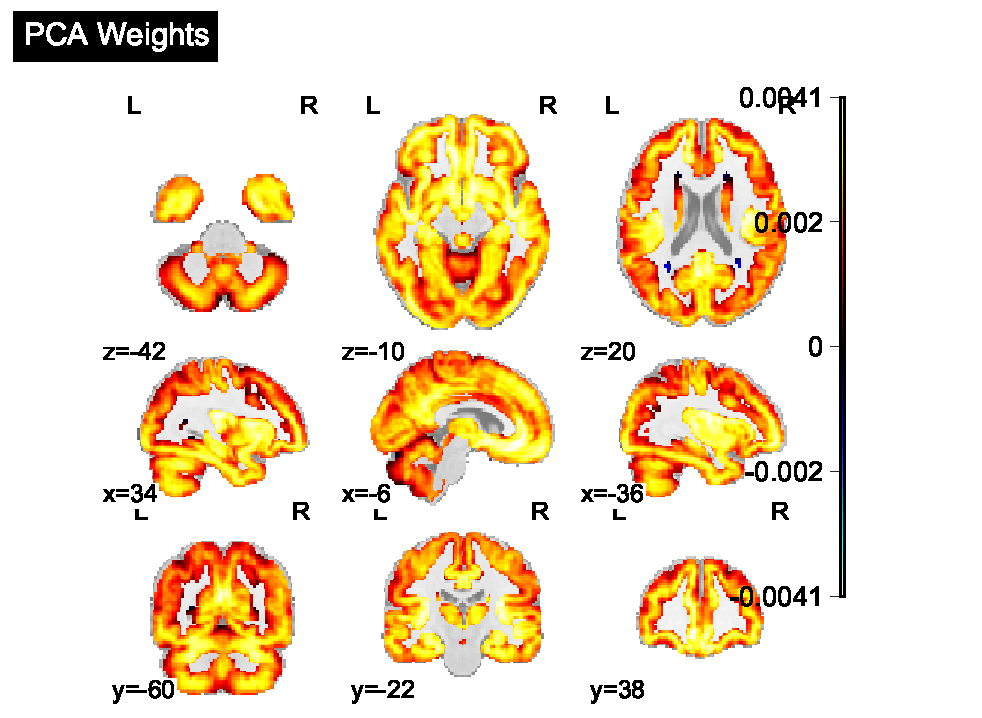
\includegraphics[width=0.45\linewidth]{figures/adni/PCA brain weights mosaic}
    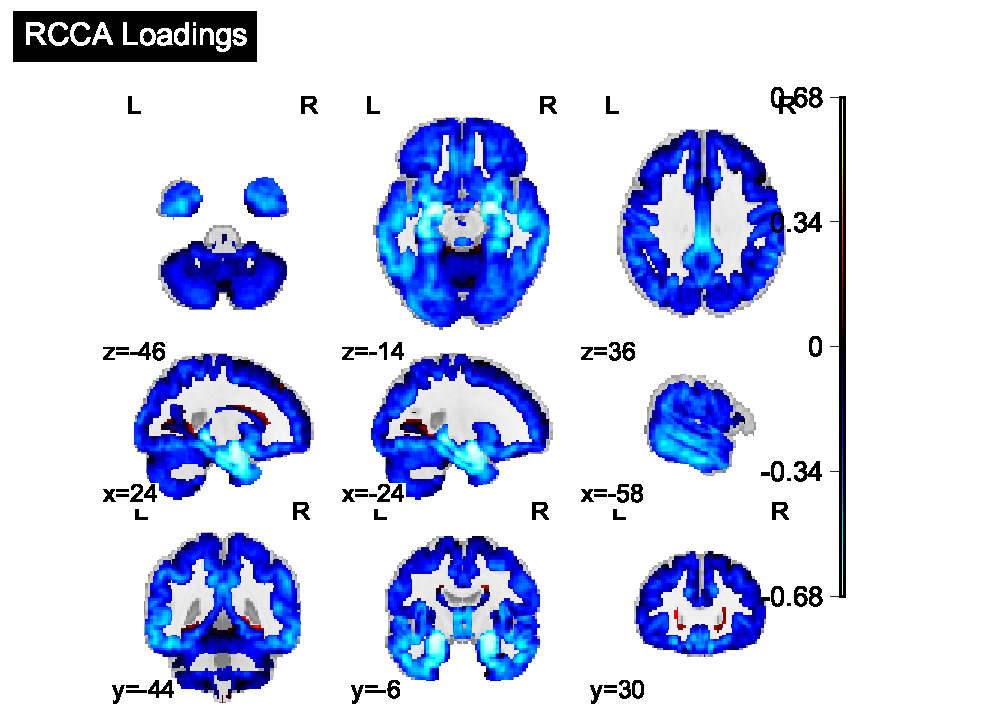
\includegraphics[width=0.45\linewidth]{figures/adni/RCCA brain loadings mosaic}
    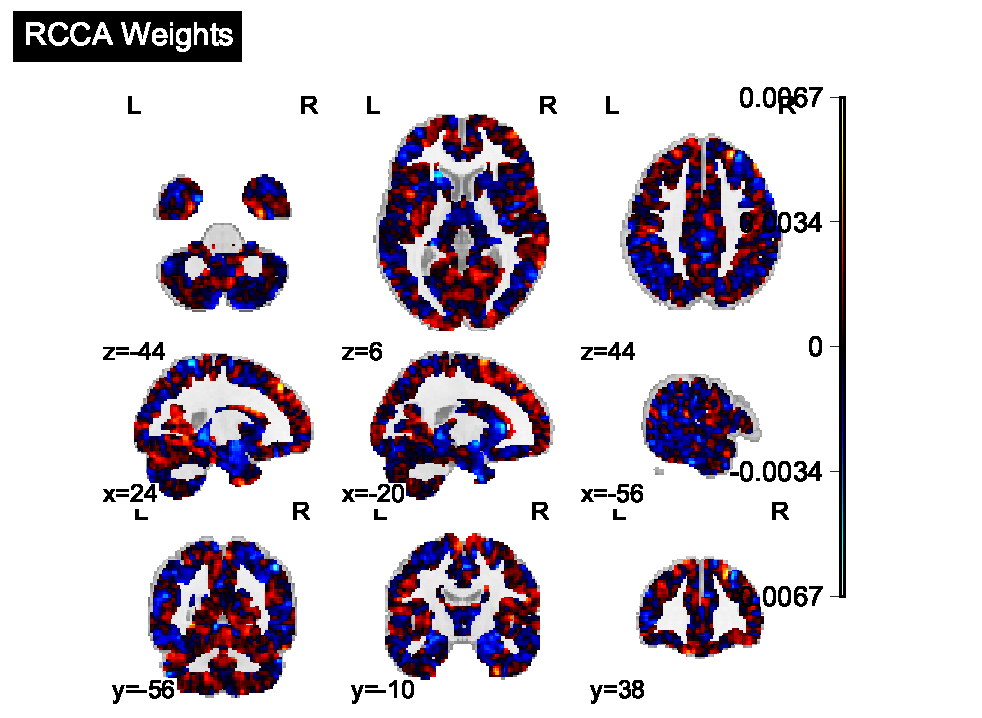
\includegraphics[width=0.45\linewidth]{figures/adni/RCCA brain weights mosaic}
    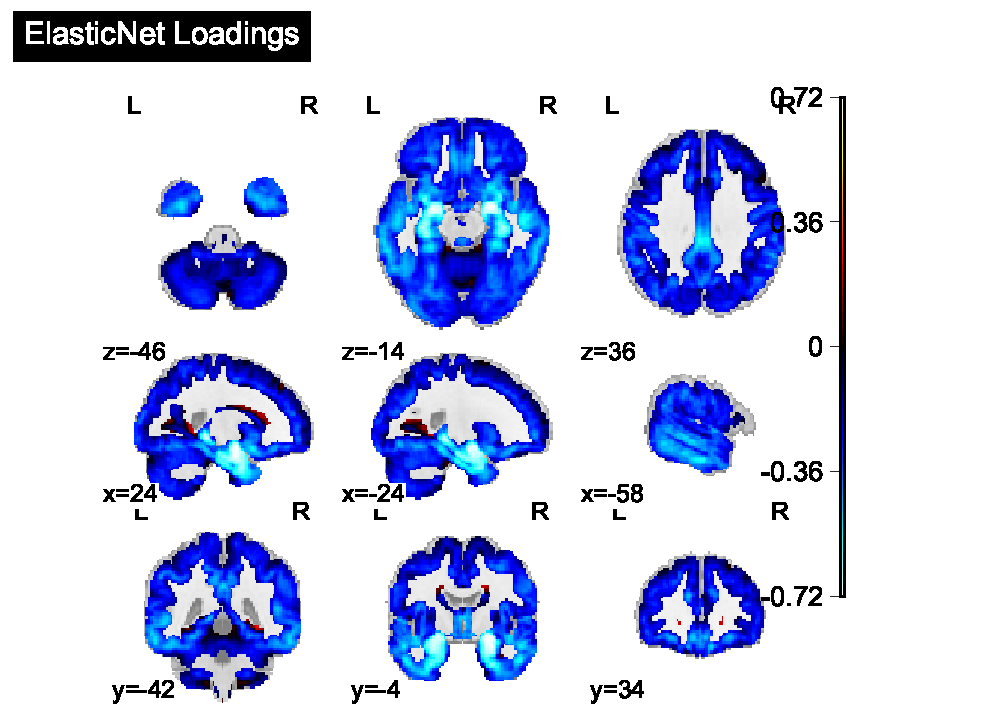
\includegraphics[width=0.45\linewidth]{figures/adni/ElasticNet brain loadings mosaic}
    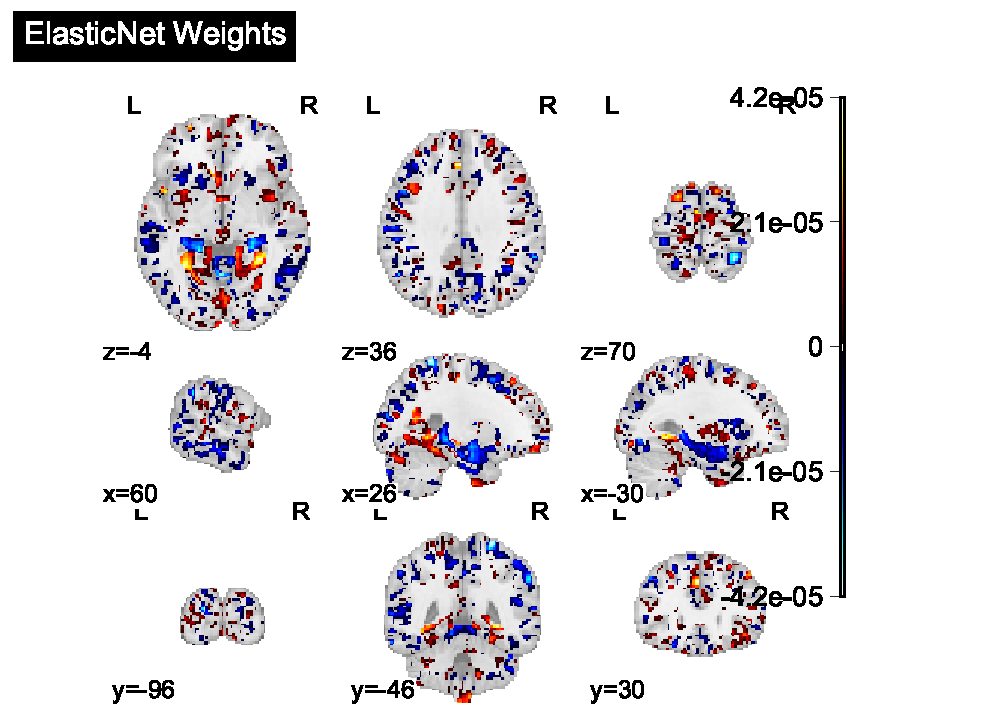
\includegraphics[width=0.45\linewidth]{figures/adni/ElasticNet brain weights mosaic}
    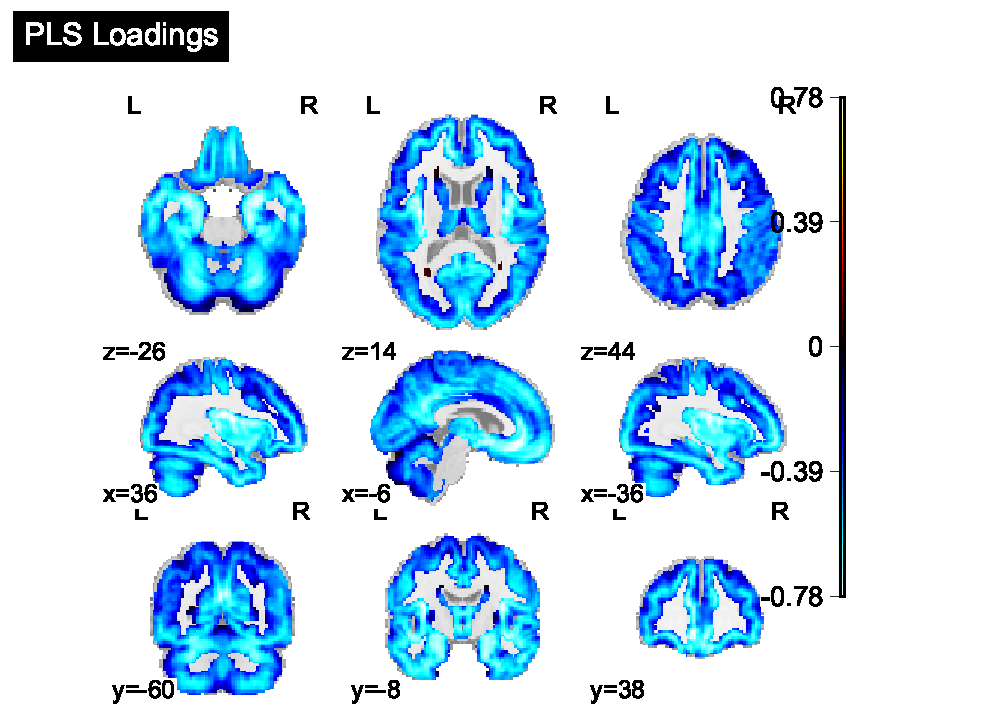
\includegraphics[width=0.45\linewidth]{figures/adni/PLS brain loadings mosaic}
    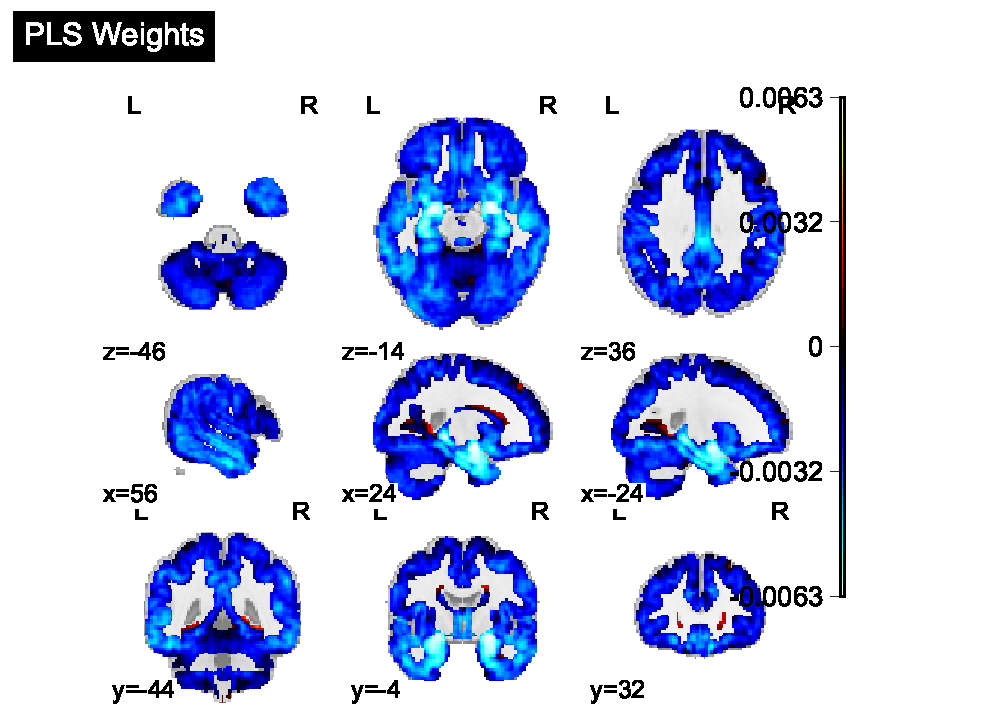
\includegraphics[width=0.45\linewidth]{figures/adni/PLS brain weights mosaic}
    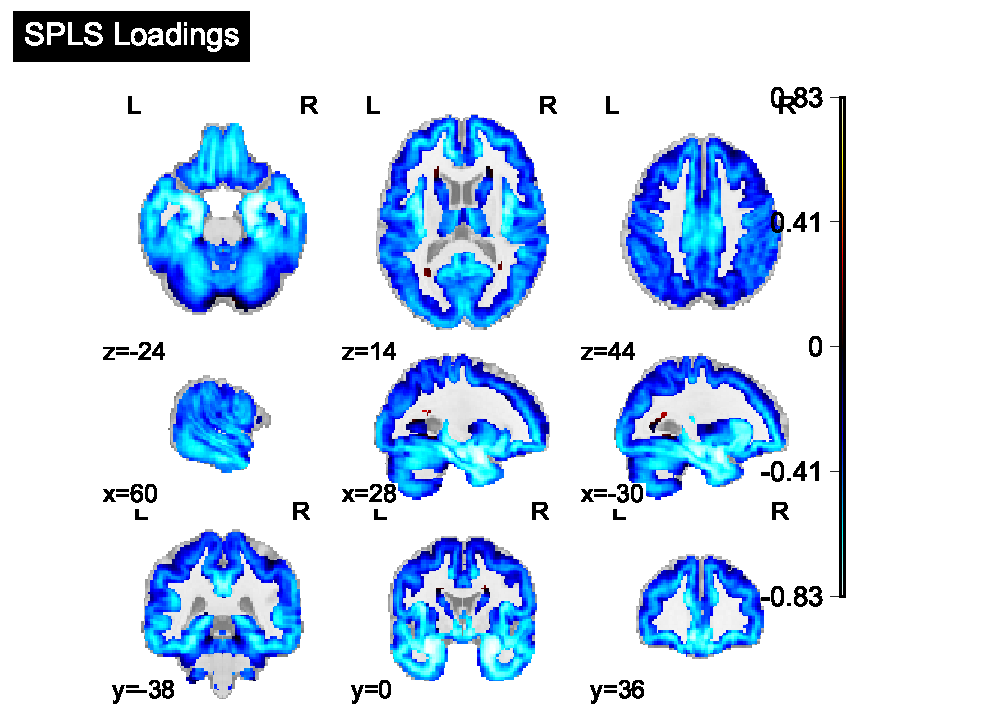
\includegraphics[width=0.45\linewidth]{figures/adni/SPLS brain loadings mosaic}
    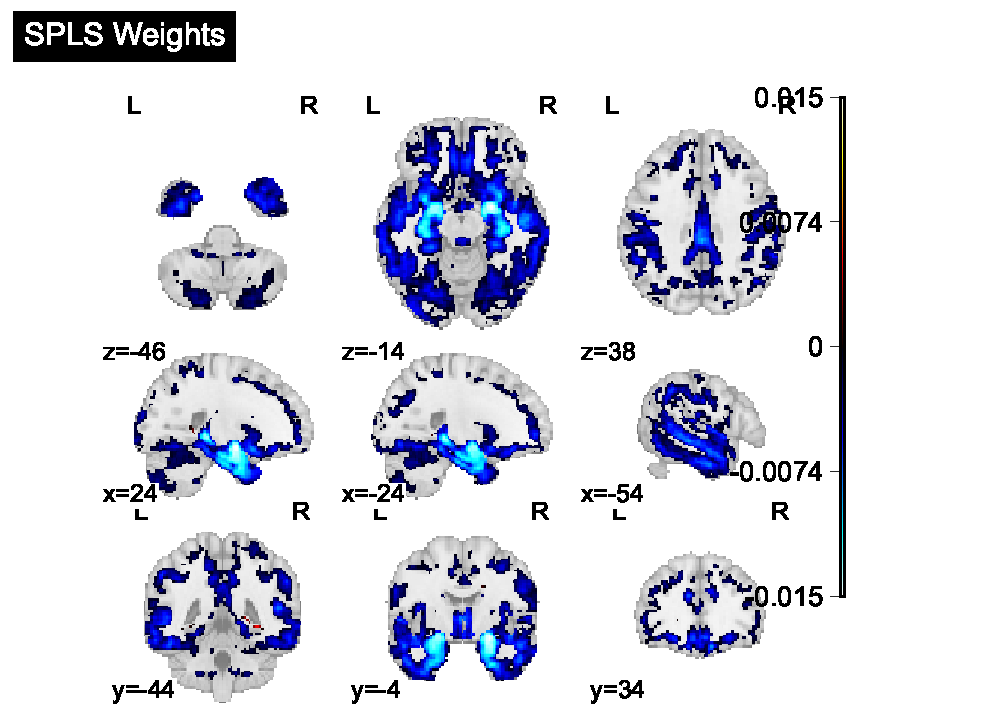
\includegraphics[width=0.45\linewidth]{figures/adni/SPLS brain weights mosaic}
    \caption{Statistical maps of brain structure \gls{loadings} and \gls{weights} for each model.}\label{fig:adni-brain}
\end{figure}